\documentclass[11pt,usenames,dvipsnames,svgnames,x11names]{beamer} 

\usetheme{Warsaw}
\usepackage{amssymb,amsmath,amsthm,amsfonts}                    
\usecolortheme{whale} 
\setbeamertemplate{navigation symbols}{}
\usepackage[utf8]{inputenc} 
\usepackage{polski}
\usepackage{tikz}
\usepackage{subfigure}
\usepackage{setspace}
\usepackage{savesym}
\savesymbol{arc}
\usepackage{color}
\usepackage{xcolor}
\usepackage{pict2e}
\usepackage{epstopdf}
\usepackage{caption}
\usepackage{graphicx}
\usepackage{pict2e}
\usepackage{epstopdf}
\usepackage{geometry}
\usepackage{mathabx}
\usepackage[normalem]{ulem}

\date{15th October 2014}
\author{Marta Sommer}
\title{Displaying Uncertainty with Shading}

\theoremstyle{plain}
\newtheorem{twierdzenie}{Twierdzenie} 
\newtheorem{twierdzeniecd}{Twierdzenie cd.} 
\theoremstyle{definition}
\newtheorem{definicja}{Definicja}
\newtheorem{przyklad}{Przykład}
\newtheorem{lemat}{Lemat}
\newtheorem{wniosek}{Wniosek}
\newtheorem{oznaczenia}{Oznaczenia}
\theoremstyle{remark}
\newtheorem{uwaga}{Uwaga}
\renewcommand*{\figurename}{Figure} 

\setbeamertemplate{caption}[numbered]

\begin{document}


\begin{frame}   %tytułowa
\titlepage
\end{frame}

%%%%%%%%%%%%%%%%%%%%%%%%%%%%%%%%%%%%%%%%%%%%%%%%%%%%%%%%%%%%%%%%%%%%%%%%%%%%%%%%%%%%%%%%%%%%%%%%%%%%%%%%%%%%%%%%%%%%%

\begin{frame}
	\frametitle{Example 1}
	\begin{columns}[t]
		\column{.5\textwidth}
			\centering
			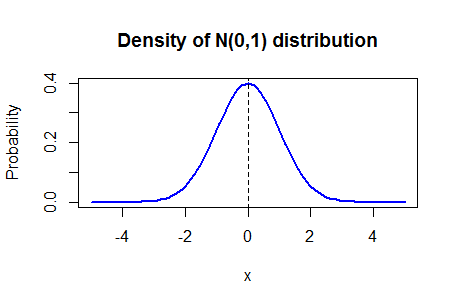
\includegraphics[width=5cm,height=4cm]{1.png}\\
			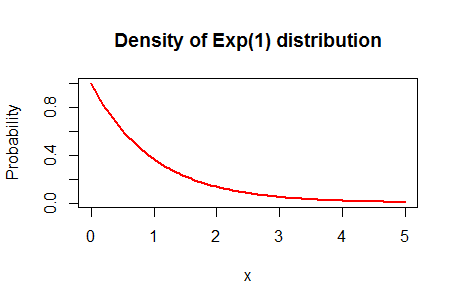
\includegraphics[width=5cm,height=4cm]{2.png}
	\column{.5\textwidth}
		\centering
		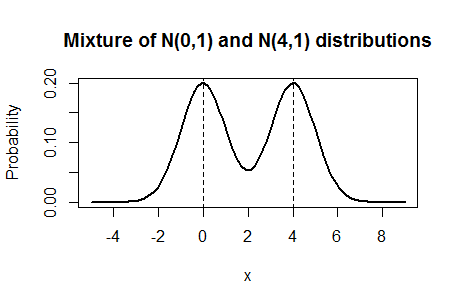
\includegraphics[width=5cm,height=4cm]{3.png}\\
		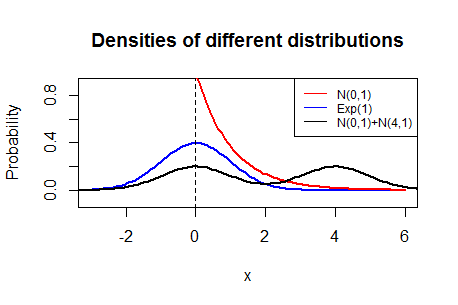
\includegraphics[width=5cm,height=4cm]{4.png}
	\end{columns}
\end{frame}

\begin{frame}
	\frametitle{Example 1 -- Point and Probability Region}
	\begin{columns}[t]
		\column{.5\textwidth}
			\centering
			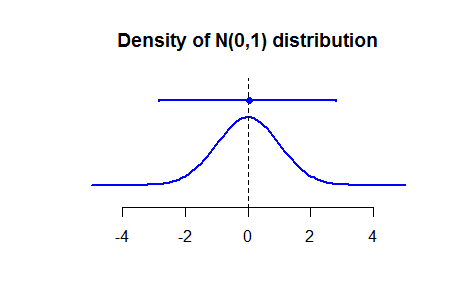
\includegraphics[width=5cm,height=4cm]{11.png}\\
			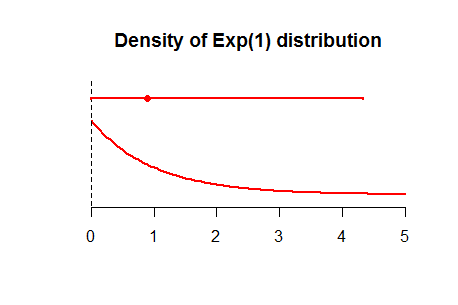
\includegraphics[width=5cm,height=4cm]{22.png}
	\column{.5\textwidth}
		\centering
		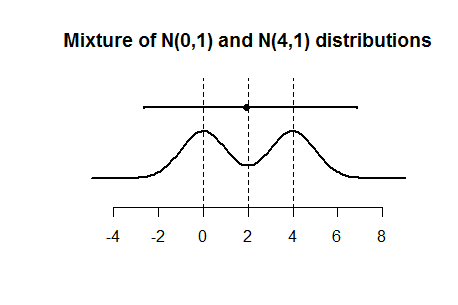
\includegraphics[width=5cm,height=4cm]{33.png}\\
		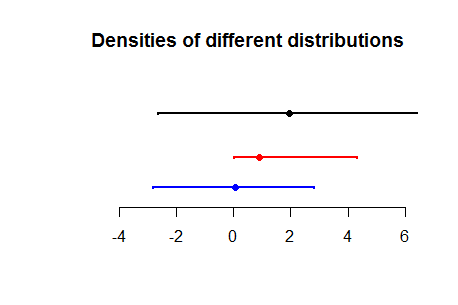
\includegraphics[width=5cm,height=4cm]{44.png}
	\end{columns}
\end{frame}

\begin{frame}
	\frametitle{Example 1 -- Point and Probability Region}
	\underline{Advantages:}	
	\begin{enumerate}
		\item easy to draw and understand,
		\item space-efficient - one dimension.
	\end{enumerate}
	\bigskip
	\underline{Disadvantages:}
	\begin{enumerate}
		\item hides information, e.g. the peaks of the mixtures of normal distributions,
		\item gives the perception that the data supports all points within the interval equally.
	\end{enumerate}
\end{frame}

\begin{frame}
	\frametitle{Example 1 -- Boxplot}
	\begin{columns}[t]
		\column{.5\textwidth}
			\centering
			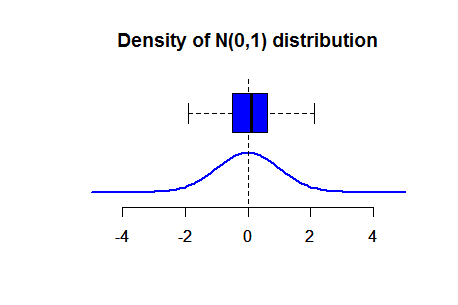
\includegraphics[width=5cm,height=4cm]{111.png}\\
			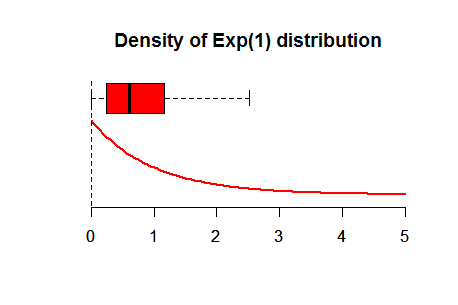
\includegraphics[width=5cm,height=4cm]{222.png}
	\column{.5\textwidth}
		\centering
		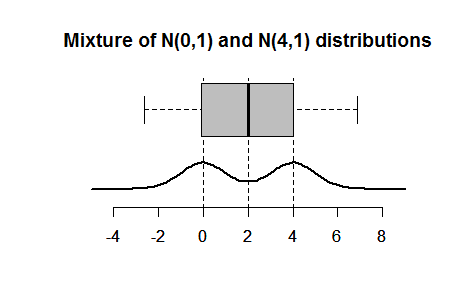
\includegraphics[width=5cm,height=4cm]{333.png}\\
		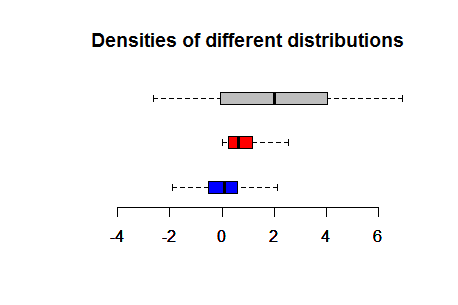
\includegraphics[width=5cm,height=4cm]{444.png}
	\end{columns}
\end{frame}

\begin{frame}
	\frametitle{Example 1 -- Boxplot}
	\underline{Advantages:}	
	\begin{enumerate}
		\item easy to draw and understand,
		\item space-efficient.
	\end{enumerate}
	\bigskip
	\underline{Disadvantages:}
	\begin{enumerate}
		\item hides information, e.g. the peaks of the mixtures of normal distributions,
		\item \sout{gives the perception that the data supports all points within the interval equally}.
	\end{enumerate}
\end{frame}

\begin{frame}
	\frametitle{Example 1 -- Box-Percentile Plot}
	\begin{columns}[t]
		\column{.5\textwidth}
			\centering
			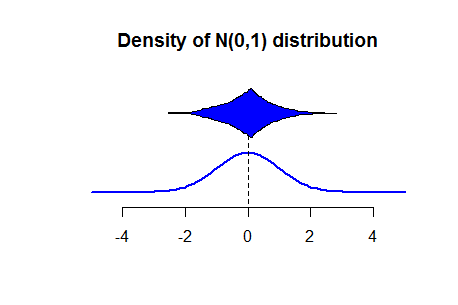
\includegraphics[width=5cm,height=4cm]{1111.png}\\
			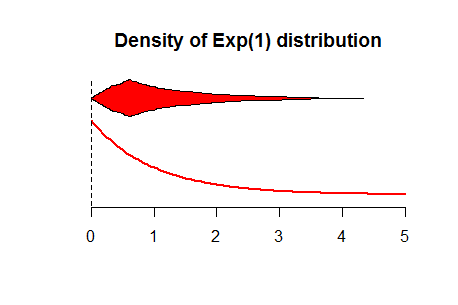
\includegraphics[width=5cm,height=4cm]{2222.png}
	\column{.5\textwidth}
		\centering
		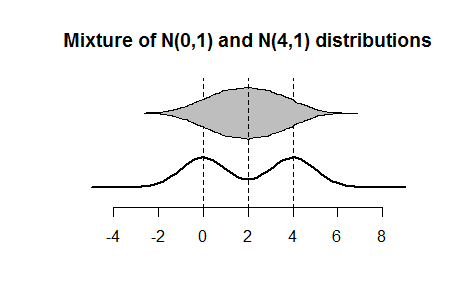
\includegraphics[width=5cm,height=4cm]{3333.png}\\
		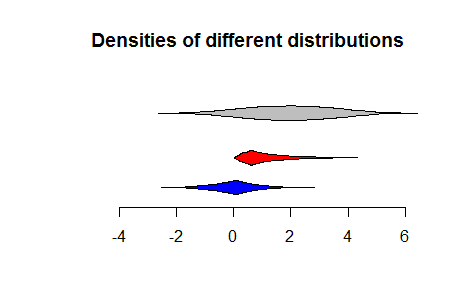
\includegraphics[width=5cm,height=4cm]{4444.png}
	\end{columns}
\end{frame}

\begin{frame}
	\frametitle{Example 1 -- Box-Percentile Plot}
	\underline{Advantages:}	
	\begin{enumerate}
		\item easy to draw and understand,
		\item \sout{space-efficient} - two dimensions.
	\end{enumerate}
	\bigskip
	\underline{Disadvantages:}
	\begin{enumerate}
		\item hides information, e.g. the peaks of the mixtures of normal distributions,
		\item \sout{gives the perception that the data supports all points within the interval equally}.
	\end{enumerate}
\end{frame}

\begin{frame}
	\frametitle{Example 1 -- Varying-Width Strips}
	\begin{columns}[t]
		\column{.5\textwidth}
			\centering
			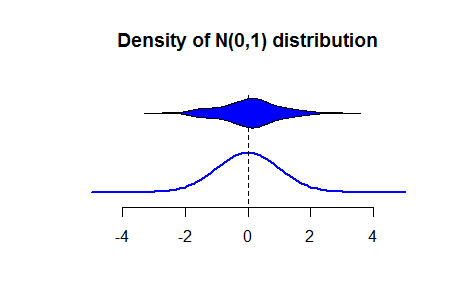
\includegraphics[width=5cm,height=4cm]{11111.png}\\
			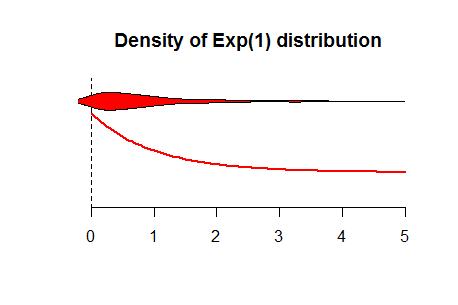
\includegraphics[width=5cm,height=4cm]{22222.png}
	\column{.5\textwidth}
		\centering
		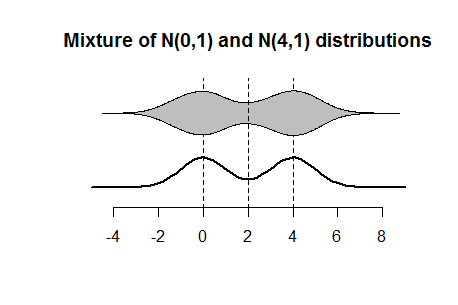
\includegraphics[width=5cm,height=4cm]{33333.png}\\
		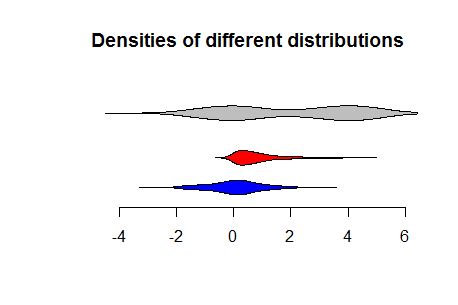
\includegraphics[width=5cm,height=4cm]{44444.png}
	\end{columns}
\end{frame}

\begin{frame}
	\frametitle{Example 1 -- Varying-Width Strips}
	\underline{Advantages:}	
	\begin{enumerate}
		\item easy to \sout{draw and} understand,
		\item \sout{space efficient} - two dimensions.
	\end{enumerate}
	\bigskip
	\underline{Disadvantages:}
	\begin{enumerate}
		\item \sout{hides information, e.g. of the mixtures of normal distributions},
		\item \sout{gives the perception that the data support all points within the interval equally}.
	\end{enumerate}
\end{frame}

\begin{frame}
	\frametitle{Example 1 -- Sectioned Density Plots}
	\begin{columns}[t]
		\column{.5\textwidth}
			\centering
			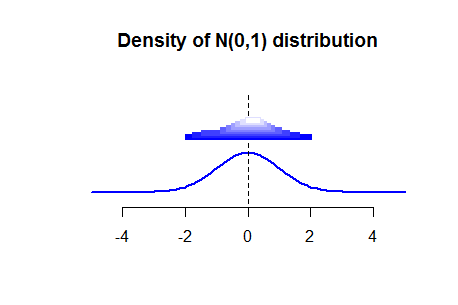
\includegraphics[width=5cm,height=4cm]{111111.png}\\
			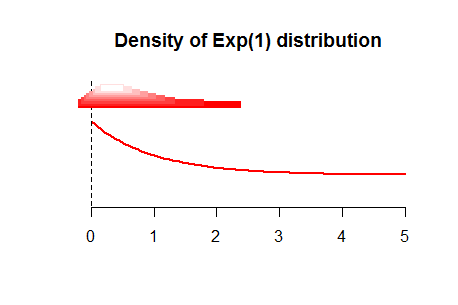
\includegraphics[width=5cm,height=4cm]{222222.png}
	\column{.5\textwidth}
		\centering
		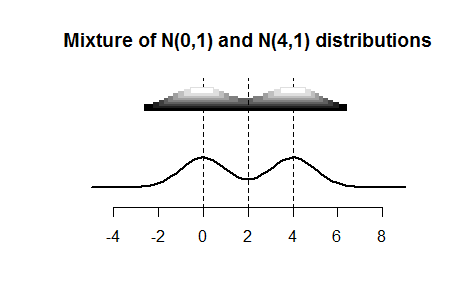
\includegraphics[width=5cm,height=4cm]{333333.png}\\
		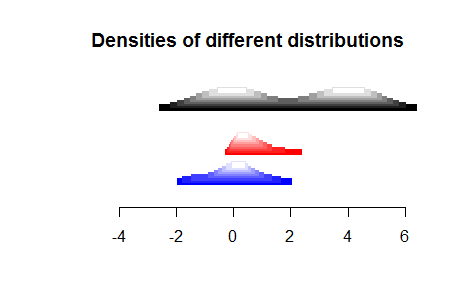
\includegraphics[width=5cm,height=4cm]{444444.png}
	\end{columns}
\end{frame}

\begin{frame}
	\frametitle{Example 1 -- Sectioned Density Plots}
	\underline{Advantages:}	
	\begin{enumerate}
		\item easy to \sout{draw and} understand,
		\item \sout{space-efficient} - two dimensions.
	\end{enumerate}
	\bigskip
	\underline{Disadvantages:}
	\begin{enumerate}
		\item \sout{hides information, e.g. the peaks of the mixtures of normal distributions},
		\item \sout{gives the perception that the data supports all points within the interval equally}.
	\end{enumerate}
\end{frame}

\begin{frame}
	\frametitle{Example 1 -- Density Strips}
	\begin{columns}[t]
		\column{.5\textwidth}
			\centering
			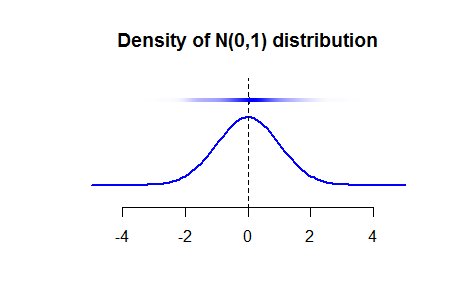
\includegraphics[width=5cm,height=4cm]{1111111.png}\\
			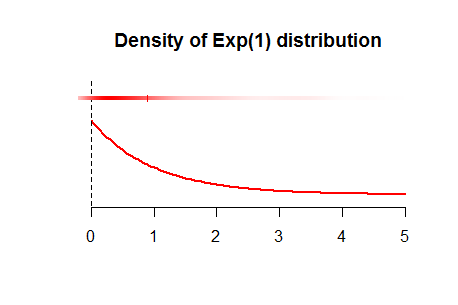
\includegraphics[width=5cm,height=4cm]{2222222.png}
	\column{.5\textwidth}
		\centering
		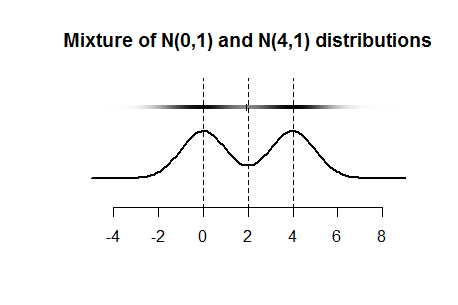
\includegraphics[width=5cm,height=4cm]{3333333.png}\\
		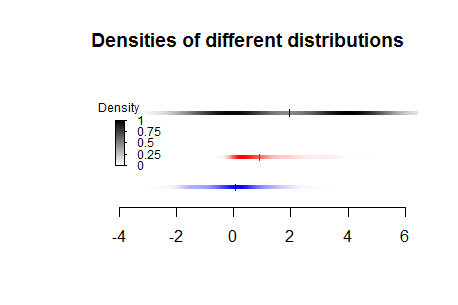
\includegraphics[width=5cm,height=4cm]{4444444.png}
	\end{columns}
\end{frame}

\begin{frame}
	\frametitle{Example 1 -- Density Strips}
	\underline{Advantages:}	
	\begin{enumerate}
		\item easy to \sout{draw and} understand,
		\item space-efficient - \underline{one dimension}.
	\end{enumerate}
	\bigskip
	\underline{Disadvantages:}
	\begin{enumerate}
		\item \sout{hides information, e.g. the peaks of the mixtures of normal distributions},
		\item \sout{gives the perception that the data support all points within the interval equally}.
	\end{enumerate}
\end{frame}

\begin{frame}
	\frametitle{Example 1 -- Summary}
	\begin{columns}[t]
		\column{.33\textwidth}
			\centering
			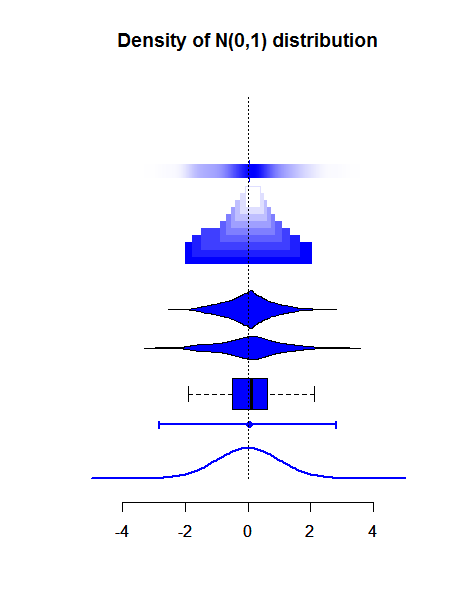
\includegraphics[width=3.5cm,height=5cm]{a.png}
		\column{.33\textwidth}
			\centering
			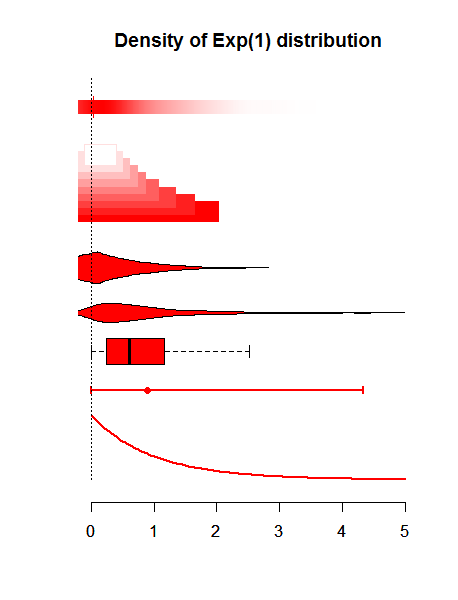
\includegraphics[width=3.5cm,height=5cm]{b.png}
		\column{.33\textwidth}
			\centering
			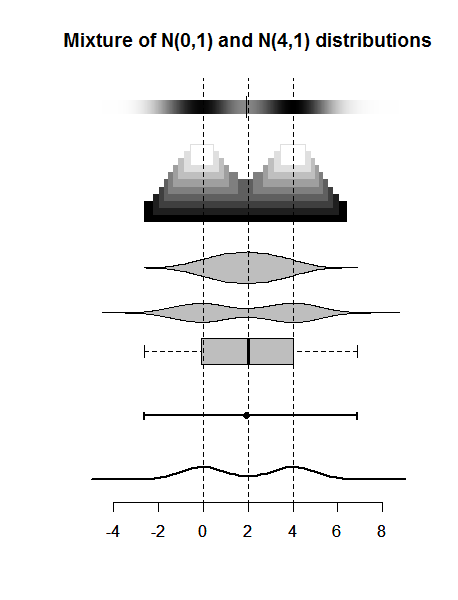
\includegraphics[width=3.5cm,height=5cm]{c.png}
	\end{columns}
\end{frame}

\begin{frame}
	\frametitle{How to Draw Density Strips?}
	
	RGB -- \colorbox{red}{red}-\colorbox{green}{green}-\colorbox{blue}{blue} model
	
	\bigskip
	
	$R,G,B \in \lbrace 0,\ldots,255 \rbrace$
	
	\bigskip
	
	$(0,0,0)$ -- \colorbox{black}{\color{white}{black}}
	
	\bigskip
	
	$(255,255,255)$ -- \fcolorbox{black}{white}{white}
	
	\bigskip
	
	Shades of \colorbox{lightgray}{grey} have equal levels of red, green and blue.
	
\end{frame}

\begin{frame}
	\frametitle{How to Draw Density Strips?}
	
	Grey level for a density $f()$ at point $x$ is the nearest integer to:
	
	$$ \left(1-\dfrac{f(x)}{f(x_0)}\right)\cdot 255, $$
	
	where $x_0$ is the mode.
	
	\bigskip
	
	If color display is available, then:
	
	$$ p\times (c_R, c_G, c_B) + (1-p)\times(255,255,255), $$

	where $p=\dfrac{f(x)}{f(x_0)}$ and $(c_R, c_G, c_B)$ is a certain dark colour chosen for the maximum density.
	
\end{frame}

\begin{frame}
	\frametitle{How to Draw Density Strips?}
	

	\textcolor{gray}{Once again:}
	
	\textcolor{gray}{$$ p\times (c_R, c_G, c_B) + (1-p)\times(255,255,255), $$}

	\textcolor{gray}{where $p=\dfrac{f(x)}{f(x_0)}$, $p\in[0,1].$}
	
	\bigskip
	
	\underline{Gamma correction:}
	
	$$ p^\gamma\times (c_R, c_G, c_B) + (1-p^\gamma)\times(255,255,255), $$	
	
	where $\gamma>0$.
	
	\bigskip
	
	Setting $\gamma<1$ will darken the tails of the distribution.
	
	\bigskip
	
	Setting $\gamma>1$ will shorten the black area around the peak.	
		
	
\end{frame}

\begin{frame}
	\frametitle{Example 2 -- Multiple Regression}
	\centering
	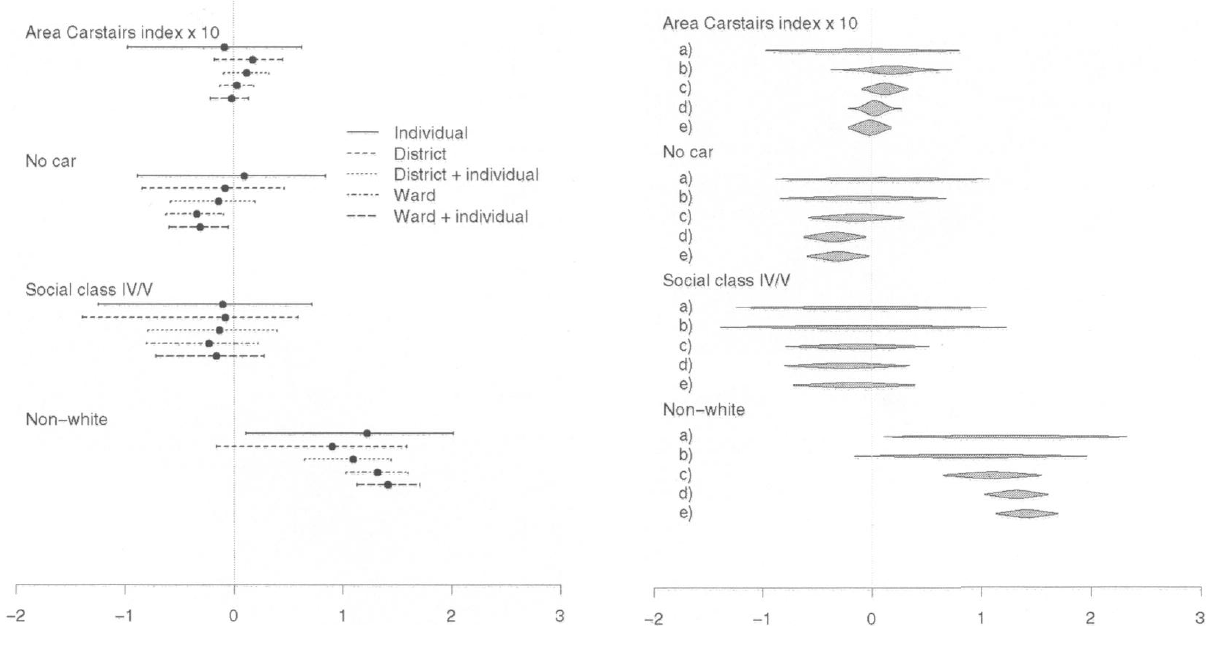
\includegraphics[width=\textwidth]{ee.png}
\end{frame}

\begin{frame}
	\frametitle{Example 2 -- Multiple Regression}
	\centering
	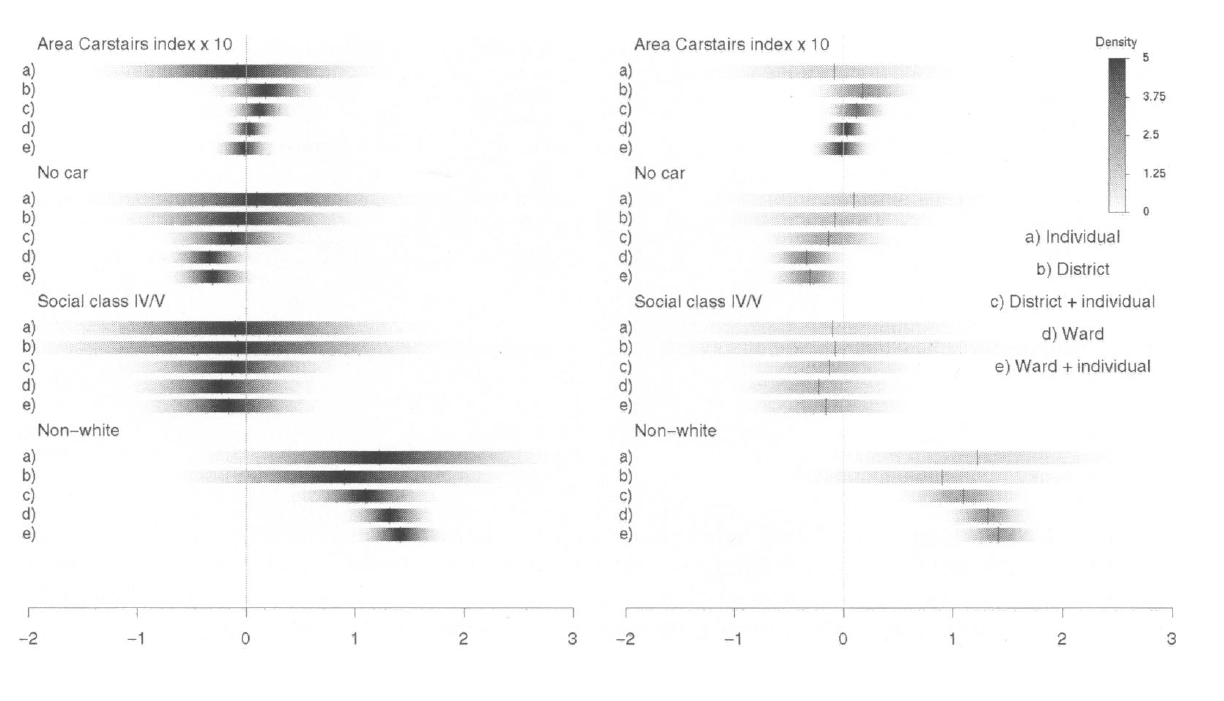
\includegraphics[width=\textwidth]{eee.png}
\end{frame}

\begin{frame}
	\frametitle{Example 3 -- Meta-Analysis}
	\centering
	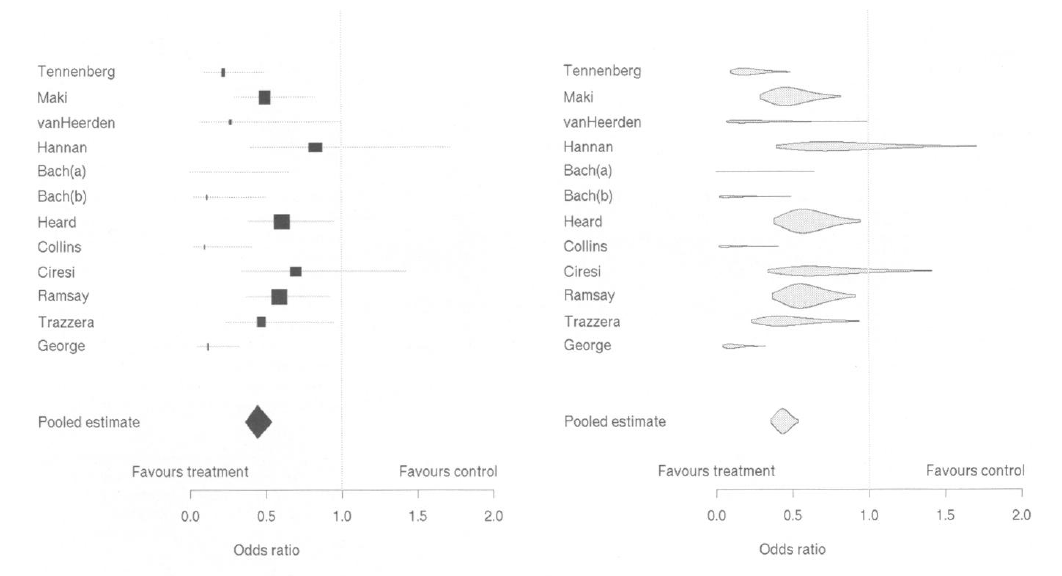
\includegraphics[width=\textwidth]{ff.png}
\end{frame}

\begin{frame}
	\frametitle{Example 3 -- Meta-Analysis}
	\centering
	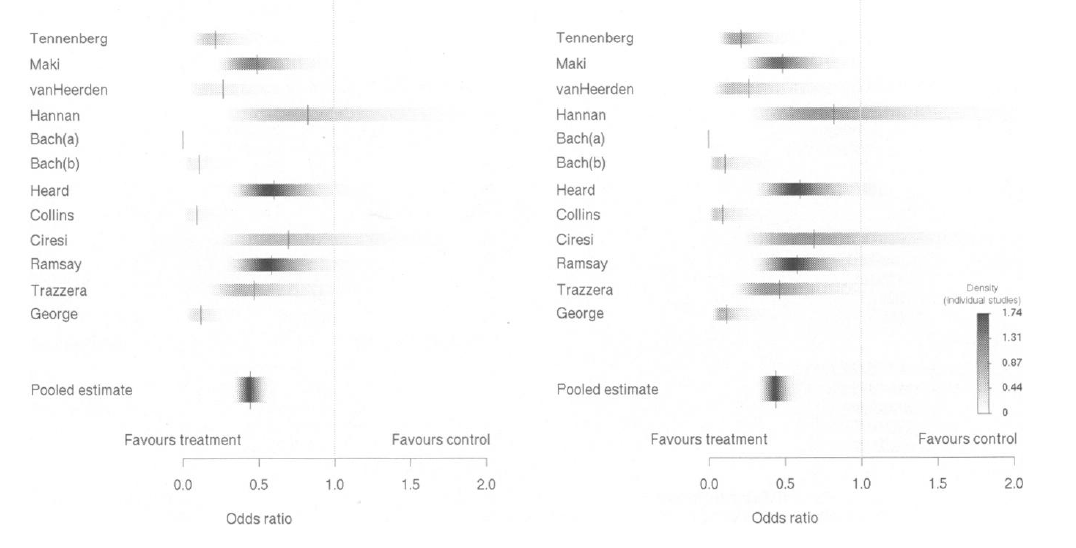
\includegraphics[width=\textwidth]{fff.png}
\end{frame}

\begin{frame}
	\frametitle{Example 4 -- Survival Analysis}
	\begin{columns}[t]
		\column{\textwidth}
			\centering
			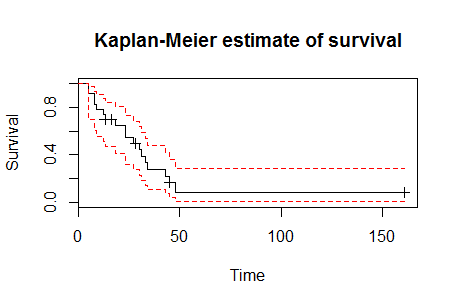
\includegraphics[width=8cm,height=4.1cm]{h.png}\\
			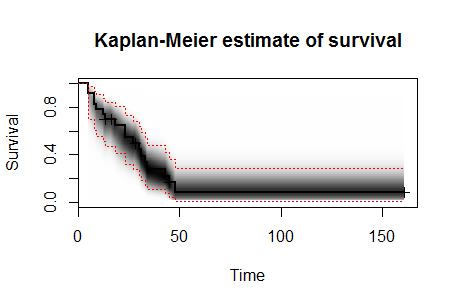
\includegraphics[width=8cm,height=4.1cm]{hh.png}
	\end{columns}
\end{frame}

\begin{frame}
	\frametitle{Example 5 -- Forecasting}
	\centering
	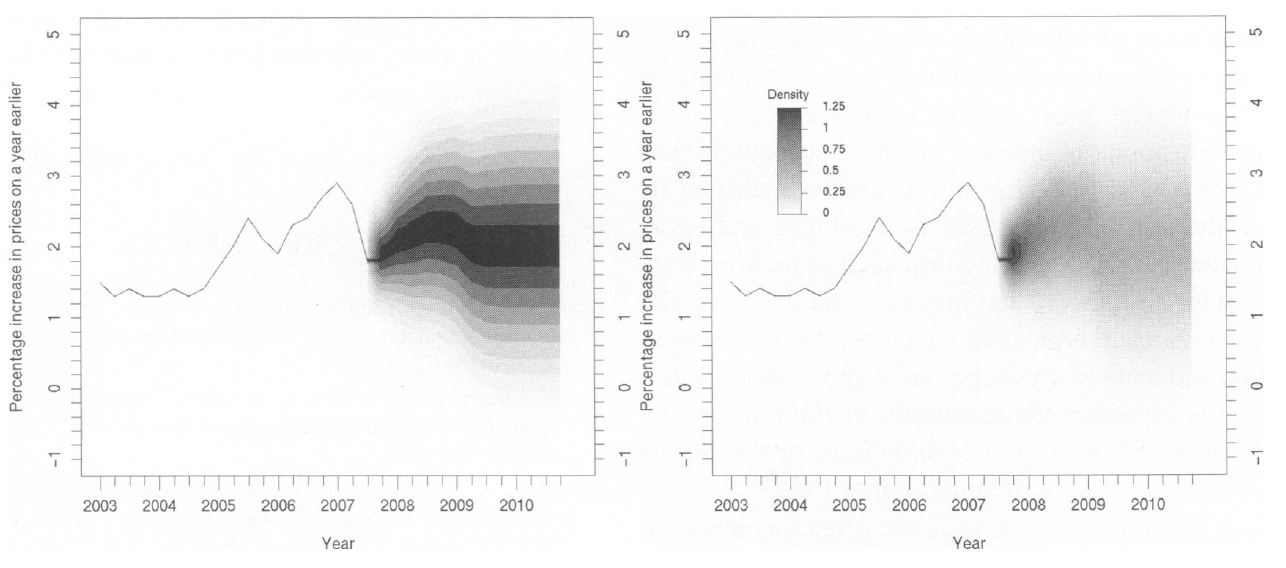
\includegraphics[width=\textwidth]{z.png}
\end{frame}

\begin{frame}
	\frametitle{Implementation in R}
	
	R package \fcolorbox{black}{white}{\texttt{denstrip}}. 
	
	\bigskip
	
	Functions:
	\begin{enumerate}
		\item \texttt{cistrip()}
		\item \texttt{vwstrip()}
		\item \texttt{bpstrip()}
		\item \texttt{sectioned.density()}
		\item \texttt{denstrip()}
	\end{enumerate}
	 	
	
\end{frame}

\begin{frame}
	\frametitle{References}
	\begin{thebibliography}{9}
		\bibitem{} Jackson, Christopher H. Displaying Uncertainty with Shading, \emph{The American Statistician} 2008, no. 62, p. 340--347.\\
		\bibitem{} \emph{http://CRAN.R-project.org/package=denstrip}
	\end{thebibliography}
\end{frame}


\end{document}
